%%
%% Automatically generated file from DocOnce source
%% (https://github.com/hplgit/doconce/)
%%
%%


%-------------------- begin preamble ----------------------

\documentclass[%
oneside,                 % oneside: electronic viewing, twoside: printing
final,                   % draft: marks overfull hboxes, figures with paths
10pt]{article}

\listfiles               %  print all files needed to compile this document

\usepackage{relsize,makeidx,color,setspace,amsmath,amsfonts,amssymb}
\usepackage[table]{xcolor}
\usepackage{bm,ltablex,microtype}

\usepackage[pdftex]{graphicx}

\usepackage[T1]{fontenc}
%\usepackage[latin1]{inputenc}
\usepackage{ucs}
\usepackage[utf8x]{inputenc}

\usepackage{lmodern}         % Latin Modern fonts derived from Computer Modern

% Hyperlinks in PDF:
\definecolor{linkcolor}{rgb}{0,0,0.4}
\usepackage{hyperref}
\hypersetup{
    breaklinks=true,
    colorlinks=true,
    linkcolor=linkcolor,
    urlcolor=linkcolor,
    citecolor=black,
    filecolor=black,
    %filecolor=blue,
    pdfmenubar=true,
    pdftoolbar=true,
    bookmarksdepth=3   % Uncomment (and tweak) for PDF bookmarks with more levels than the TOC
    }
%\hyperbaseurl{}   % hyperlinks are relative to this root

\setcounter{tocdepth}{2}  % levels in table of contents

% Tricks for having figures close to where they are defined:
% 1. define less restrictive rules for where to put figures
\setcounter{topnumber}{2}
\setcounter{bottomnumber}{2}
\setcounter{totalnumber}{4}
\renewcommand{\topfraction}{0.95}
\renewcommand{\bottomfraction}{0.95}
\renewcommand{\textfraction}{0}
\renewcommand{\floatpagefraction}{0.75}
% floatpagefraction must always be less than topfraction!
% 2. ensure all figures are flushed before next section
\usepackage[section]{placeins}
% 3. enable begin{figure}[H] (often leads to ugly pagebreaks)
%\usepackage{float}\restylefloat{figure}

\usepackage[framemethod=TikZ]{mdframed}

% --- begin definitions of admonition environments ---

% Admonition style "mdfbox" is an oval colored box based on mdframed
% "notice" admon
\colorlet{mdfbox_notice_background}{gray!5}
\newmdenv[
  skipabove=15pt,
  skipbelow=15pt,
  outerlinewidth=0,
  backgroundcolor=mdfbox_notice_background,
  linecolor=black,
  linewidth=2pt,       % frame thickness
  frametitlebackgroundcolor=mdfbox_notice_background,
  frametitlerule=true,
  frametitlefont=\normalfont\bfseries,
  shadow=false,        % frame shadow?
  shadowsize=11pt,
  leftmargin=0,
  rightmargin=0,
  roundcorner=5,
  needspace=0pt,
]{notice_mdfboxmdframed}

\newenvironment{notice_mdfboxadmon}[1][]{
\begin{notice_mdfboxmdframed}[frametitle=#1]
}
{
\end{notice_mdfboxmdframed}
}

% Admonition style "mdfbox" is an oval colored box based on mdframed
% "summary" admon
\colorlet{mdfbox_summary_background}{gray!5}
\newmdenv[
  skipabove=15pt,
  skipbelow=15pt,
  outerlinewidth=0,
  backgroundcolor=mdfbox_summary_background,
  linecolor=black,
  linewidth=2pt,       % frame thickness
  frametitlebackgroundcolor=mdfbox_summary_background,
  frametitlerule=true,
  frametitlefont=\normalfont\bfseries,
  shadow=false,        % frame shadow?
  shadowsize=11pt,
  leftmargin=0,
  rightmargin=0,
  roundcorner=5,
  needspace=0pt,
]{summary_mdfboxmdframed}

\newenvironment{summary_mdfboxadmon}[1][]{
\begin{summary_mdfboxmdframed}[frametitle=#1]
}
{
\end{summary_mdfboxmdframed}
}

% Admonition style "mdfbox" is an oval colored box based on mdframed
% "warning" admon
\colorlet{mdfbox_warning_background}{gray!5}
\newmdenv[
  skipabove=15pt,
  skipbelow=15pt,
  outerlinewidth=0,
  backgroundcolor=mdfbox_warning_background,
  linecolor=black,
  linewidth=2pt,       % frame thickness
  frametitlebackgroundcolor=mdfbox_warning_background,
  frametitlerule=true,
  frametitlefont=\normalfont\bfseries,
  shadow=false,        % frame shadow?
  shadowsize=11pt,
  leftmargin=0,
  rightmargin=0,
  roundcorner=5,
  needspace=0pt,
]{warning_mdfboxmdframed}

\newenvironment{warning_mdfboxadmon}[1][]{
\begin{warning_mdfboxmdframed}[frametitle=#1]
}
{
\end{warning_mdfboxmdframed}
}

% Admonition style "mdfbox" is an oval colored box based on mdframed
% "question" admon
\colorlet{mdfbox_question_background}{gray!5}
\newmdenv[
  skipabove=15pt,
  skipbelow=15pt,
  outerlinewidth=0,
  backgroundcolor=mdfbox_question_background,
  linecolor=black,
  linewidth=2pt,       % frame thickness
  frametitlebackgroundcolor=mdfbox_question_background,
  frametitlerule=true,
  frametitlefont=\normalfont\bfseries,
  shadow=false,        % frame shadow?
  shadowsize=11pt,
  leftmargin=0,
  rightmargin=0,
  roundcorner=5,
  needspace=0pt,
]{question_mdfboxmdframed}

\newenvironment{question_mdfboxadmon}[1][]{
\begin{question_mdfboxmdframed}[frametitle=#1]
}
{
\end{question_mdfboxmdframed}
}

% Admonition style "mdfbox" is an oval colored box based on mdframed
% "block" admon
\colorlet{mdfbox_block_background}{gray!5}
\newmdenv[
  skipabove=15pt,
  skipbelow=15pt,
  outerlinewidth=0,
  backgroundcolor=mdfbox_block_background,
  linecolor=black,
  linewidth=2pt,       % frame thickness
  frametitlebackgroundcolor=mdfbox_block_background,
  frametitlerule=true,
  frametitlefont=\normalfont\bfseries,
  shadow=false,        % frame shadow?
  shadowsize=11pt,
  leftmargin=0,
  rightmargin=0,
  roundcorner=5,
  needspace=0pt,
]{block_mdfboxmdframed}

\newenvironment{block_mdfboxadmon}[1][]{
\begin{block_mdfboxmdframed}[frametitle=#1]
}
{
\end{block_mdfboxmdframed}
}

% --- end of definitions of admonition environments ---

% prevent orhpans and widows
\clubpenalty = 10000
\widowpenalty = 10000

% --- end of standard preamble for documents ---


% insert custom LaTeX commands...

\raggedbottom
\makeindex
\usepackage[totoc]{idxlayout}   % for index in the toc
\usepackage[nottoc]{tocbibind}  % for references/bibliography in the toc

%-------------------- end preamble ----------------------

\begin{document}

% matching end for #ifdef PREAMBLE

\newcommand{\exercisesection}[1]{\subsection*{#1}}


% ------------------- main content ----------------------



% ----------------- title -------------------------

\thispagestyle{empty}

\begin{center}
{\LARGE\bf
\begin{spacing}{1.25}
Machine Learning and AI in Nuclear Physics
\end{spacing}
}
\end{center}

% ----------------- author(s) -------------------------

\begin{center}
{\bf Daniel Bazin, Scott Bogner, Alexandra Gade, Heiko Hergert, Morten Hjorth-Jensen, Dean Lee, Sean Liddick, Witek Nazarewicz and Andrea Shindler}
\end{center}

    \begin{center}
% List of all institutions:
\centerline{{\small Department of Physics and Astronomy and Facility for Rare Ion Beams and National Superconducting Cyclotron Laboratory, Michigan State University, USA}}
\end{center}
    
% ----------------- end author(s) -------------------------

% --- begin date ---
\begin{center}
Talking points
\end{center}
% --- end date ---

\vspace{1cm}


% !split
\subsection{Machine Learning and AI and Nuclear Physics}

\begin{block_mdfboxadmon}[]

Artificial intelligence-based techniques, particularly in machine
learning and optimization, are increasingly being used in many areas
of experimental and theoretical physics to facilitate discovery,
accelerate data analysis and modeling efforts, and bridge different
physical and temporal scales in numerical models.

These techniques are proving to be powerful tools for advancing our
understanding; however, they are not without significant
challenges. The theoretical foundations of many tools, such as deep
learning, are poorly understood, resulting in the use of techniques
whose behavior (and misbehavior) is difficult to predict and
understand. Similarly, physicists typically use general AI techniques
that are not tailored to the needs of the experimental and theoretical
work being done. Thus, many opportunities exist for major advances
both in physical discovery using AI and in the theory of
AI. Furthermore, there are tremendous opportunities for these fields
to inform each other, for example, in creating machine learning- based
methods that must obey certain constraints by design, such as the
conservation of mass, momentum and energy.
\end{block_mdfboxadmon} % title: 





% !split
\subsection{What is Machine Learning?}

\begin{block_mdfboxadmon}[]
Machine learning is the science of giving computers the ability to
learn without being explicitly programmed.  The idea is that there
exist generic algorithms which can be used to find patterns in a broad
class of data sets without having to write code specifically for each
problem. The algorithm will build its own logic based on the data.

Machine learning is a subfield of computer science, and is closely
related to computational statistics.  It evolved from the study of
pattern recognition in artificial intelligence (AI) research, and has
made contributions to AI tasks like computer vision, natural language
processing and speech recognition. It has also, especially in later
years, found applications in a wide variety of other areas, including
bioinformatics, economy, physics, finance and marketing.
\end{block_mdfboxadmon} % title: 






% !split
\subsection{A new world}

\begin{block_mdfboxadmon}[]
Machine learning (ML) is an extremely rich field, in spite of its young age. The
increases we have seen during the last three decades in computational
capabilities have been followed by developments of methods and
techniques for analyzing and handling large date sets, relying heavily
on statistics, computer science and mathematics.  The field is rather
new and developing rapidly. 

Popular software packages written in Python for ML are

\begin{itemize}
\item \href{{http://scikit-learn.org/stable/}}{Scikit-learn}, 

\item \href{{https://www.tensorflow.org/}}{Tensorflow},

\item \href{{http://pytorch.org/}}{PyTorch}

\item \href{{https://keras.io/}}{Keras},
\end{itemize}

\noindent
and more. These are all freely available at their respective GitHub sites. They 
encompass communities of developers in the thousands or more. And the number
of code developers and contributors keeps increasing.
\end{block_mdfboxadmon} % title: 



% !split
\subsection{Lots of room for creativity}

\begin{block_mdfboxadmon}[]
Not all the
algorithms and methods can be given a rigorous mathematical
justification, opening up thereby for experimenting
and trial and error and thereby exciting new developments.
\end{block_mdfboxadmon} % title: 




\begin{block_mdfboxadmon}[]
A solid command of linear algebra, multivariate theory, 
probability theory, statistical data analysis, optimization algorithms, 
understanding errors and Monte Carlo methods is important in order to understand many of the 
various algorithms and methods.
\end{block_mdfboxadmon} % title: 




% !split
\subsection{Types of Machine Learning}


\begin{block_mdfboxadmon}[]
The approaches to machine learning are many, but are often split into two main categories. 
In \emph{supervised learning} we know the answer to a problem,
and let the computer deduce the logic behind it. On the other hand, \emph{unsupervised learning}
is a method for finding patterns and relationship in data sets without any prior knowledge of the system.
Some authours also operate with a third category, namely \emph{reinforcement learning}. This is a paradigm 
of learning inspired by behavioural psychology, where learning is achieved by trial-and-error, 
solely from rewards and punishment.

Another way to categorize machine learning tasks is to consider the desired output of a system.
Some of the most common tasks are:

\begin{itemize}
  \item Classification: Outputs are divided into two or more classes. The goal is to   produce a model that assigns inputs into one of these classes. An example is to identify  digits based on pictures of hand-written ones. Classification is typically supervised learning.

  \item Regression: Finding a functional relationship between an input data set and a reference data set.   The goal is to construct a function that maps input data to continuous output values.

  \item Clustering: Data are divided into groups with certain common traits, without knowing the different groups beforehand.  It is thus a form of unsupervised learning.
\end{itemize}

\noindent
\end{block_mdfboxadmon} % title: 




% !split
\subsection{Why Machine Learning and Nuclear Physics, Motivation}

Techniques based on artificial intelligence (AI), particularly in
machine learning (ML) and optimization, are increasingly being used in
many areas of experimental and theoretical physics to facilitate
discovery, accelerate data analysis and modeling efforts, and bridge
different physical and temporal scales in numerical models. These 
techniques are proving to be powerful tools for advancing our physical
understanding; however, they are not without significant challenges
of their own. The theoretical foundations of many AI tools, such as
deep learning, are poorly understood, resulting in the use of
techniques whose behavior (and misbehavior) is difficult to predict
and understand. Similarly, physicists typically use general AI
techniques that are not tailored to the needs of the experimental and
theoretical work being done. As a consequence, there is a profound
need for major advances both in the ways that AI techniques are used
in physics and in the theoretical foundations of AI
methods. Furthermore, there are tremendous opportunities for these
fields to inform each other, for example, in creating ML-based
methods that must obey physical constraints by design, e.g.,
conservation of energy.


% !split
\subsection{Further Motivation}

Physics has historically been on the forefront of the data revolution,
and the future will be no different. Upcoming expansions to the
Large Hadron Collider will increase data rates by an order of
magnitude past their previous peak, and high-current nuclear physics
facilities such as the DOE’s Facility for Rare Isotope Beams will also
have incredibly high rates of data production. These laboratories and experiments
will produce large and rich (but
complicated) time-sequence datasets. In theoretical physics, the need
to address such experiments requires sophisticated, multiphysics
numerical simulations that span a wide range of spatial and temporal
scales, physical models (e.g., particle vs.~continuum ap-
proximations). Even with the advent of exascale
computing, approximations must be made in order to make the problems
computationally tractable.


% !split
\subsection{A simple perspective on the interface between ML and Physics}



\vspace{6mm}

% inline figure
\centerline{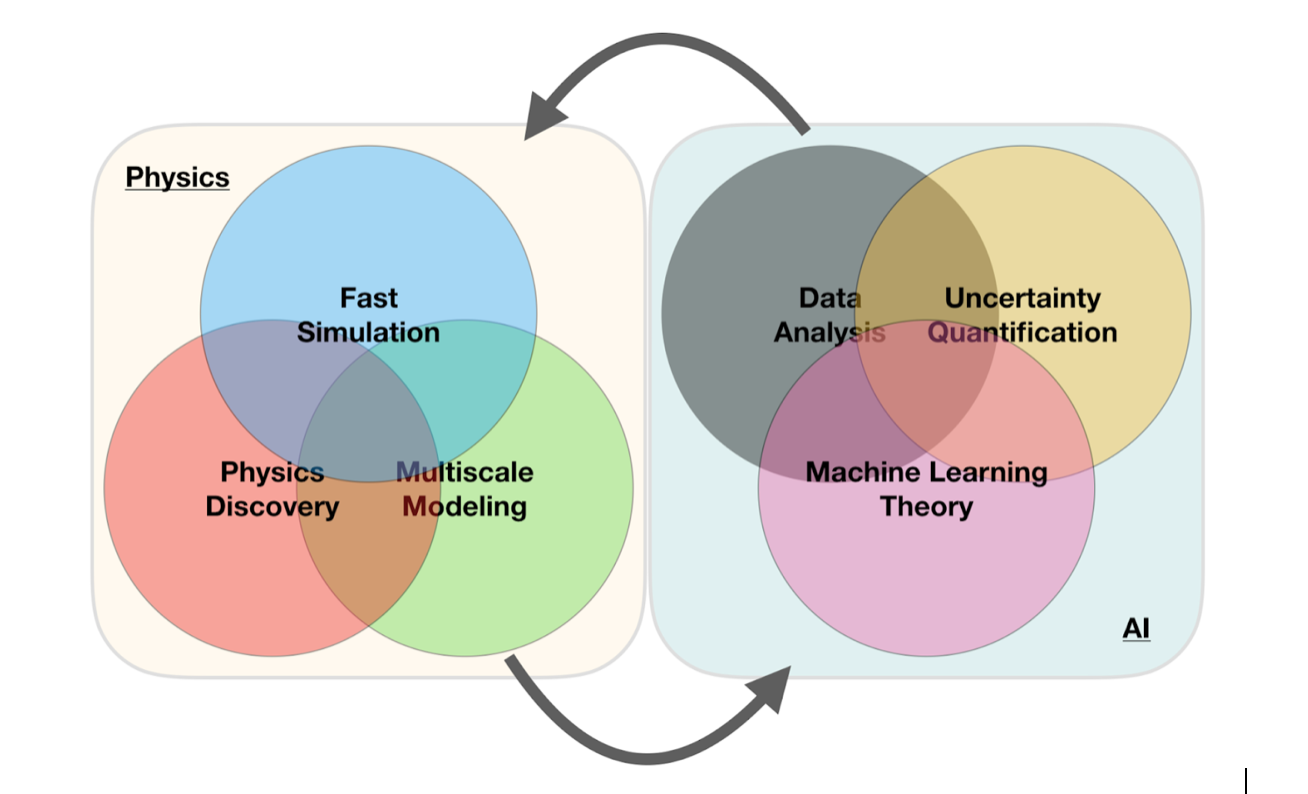
\includegraphics[width=0.9\linewidth]{figures/mlimage.png}}

\vspace{6mm}




% !split
\subsection{ML in Nuclear Physics, Examples}

The large amount of degrees of freedom pertain to both theory and experiemtn in nuclear physics. With increasingly complicated experiments that produce large amounts data, automated classification of events becomes increasingly important. Here, deep learning methods offer a plethora of interesting research avenues. 

\begin{itemize}
\item Reconstruction of particle trajectories or classification of events are typical examples where ML methods are being used. However, since these data can often be extremely noisy, the precision necessary for discovery in physics requires algorithmic improvements. Research along such directions, interfacing nuclear physics with AI/ML is expected to play a significant role in physics discoveries related to new facilities.  The treatment of corrupted data in imaging and image processing is also a relevant topic. 

\item Design of detectors represents an important area of applications for ML/AI methods in nuclear physics.

\item Many of the above classification problems have also have direct application in theoretical nuclear physics (including Lattice QCD calculations).
\end{itemize}

\noindent
% !split
\subsection{More examples}

\begin{itemize}
\item An important application of AI/L methods is to improve the estimation of bias or uncertainty due to the introduction of or lack of physical constraints in various theoretical models.

\item In theory, we expect to use AI/ML algorithms and methods to improve our knowledged about  correlations of physical model parameters in data for quantum many-body systems. Deep learning methods like Boltzmann machines and various types of Recurrent Neural networks show great promise in circumventing the exploding dimensionalities encountered in quantum mechanical many-body studies. 

\item Merging a frequentist approach (the standard path in ML theory) with a Bayesian approach, has the potential to infer better probabilitity distributions and error estimates. As an example, methods for fast Monte-Carlo- based Bayesian computation of nuclear density functionals show great promise in providing a better understanding 

\item Machine Learning and Quantum Computing is a very interesting avenue to explore.
\end{itemize}

\noindent
% !split
\subsection{Education and Work force development}

AI, ML, statistical data analysis and related areas are expected to
play an ever-increasing role in many areas, from fundamental and
applied research at universities and national laboratories to
applications and developments in both the private and the public
sectors.
Developing basic research activities in these frontier
computational technologies is thus of strategic importance for our
society’s capability to address future scientific problems. Transfer
of knowledge to other disciplines and sectors, as well as developing
lasting collaborations with partners outside the traditional
university sector, are themes we expect will benefit society at large
and that will play central roles. Nuclear Physics keeps attracting many brilliant young researchers and providing our work force with these competences and skills for solving complicated physics problems is a compelling task for our community.

More text will come.

\begin{itemize}
\item In order to develop education and training efforts that target AI and ML related methods applied to Nuclear Physics, we  organized in 2019 a four day long  FRIB-TA workshop on ML methods in Nuclear physics at the NSCL/FRIB, with more than 100 participants.

\item In 2020 several of us (Bazin, Hjorth-Jensen and Liddick) will teach a three-week long Nuclear Talent course on Machine Learning and Data Analysis applied to nuclear physics. 
\end{itemize}

\noindent
% !split
\subsection{References}

\begin{block_mdfboxadmon}[]
\begin{itemize}
\item An excellent reference, \href{{https://arxiv.org/abs/1803.08823}}{Mehta et al.} and \href{{https://www.sciencedirect.com/science/article/pii/S0370157319300766?via%3Dihub}}{Physics Reports (2019)}.

\item \href{{https://arxiv.org/abs/1903.10563}}{Machine Learning and the Physical Sciences by Carleo et al}

\item \href{{https://arxiv.org/pdf/1909.02487.pdf}}{Many-electron systems with Deep Learning}

\item \href{{https://journals.aps.org/prl/abstract/10.1103/PhysRevLett.120.156001}}{Every issue of Physical Review Letters has now one or more articles on ML}

\item \href{{https://github.com/copperwire/thesis/blob/master/main.pdf}}{Classifying Nuclear Physics  experiments from the NSCL}

\item \href{{https://github.com/bsamseth/qflow}}{Software and thesis on many-body methods and Machine Learning}

\item \href{{https://github.com/CompPhysics/MachineLearning}}{Books and lectures notes} and see also the course \href{{https://www.uio.no/studier/emner/matnat/fys/FYS-STK4155/h18/index.html}}{FYS-STK3155/4155}
\end{itemize}

\noindent
\end{block_mdfboxadmon} % title: 









% ------------------- end of main content ---------------

\end{document}

